\section{Auswertung}

\subsection{Charakteristik des Geiger-Müllerzählrohrs}

Die gemessenen Daten zur Charakteristik des Geiger-Müllerzählrohrs sind in der Tabelle \ref{tab:ogemessdaten}
angegeben. Dabei ist die Zählrate poissonverteilt und lässt sich gemäß Gleichung \ref{eqn:fehlerzählrate} berechnen.
\newline
Zunächst sollen die Messpunkte mit einem Fehlerbalken in ein Diagramm eingezeichnet werden und anschließend soll entlang des Plateau-Bereiches
eine lineare Ausgleichsgerade erstellt werden. Graphisch lässt sich der Plateau-Bereich, also der Bereich in der die Zählrate kaum zunimmt bei ansteigender angelegter Spannung, grob
als Intervall von $\SI{370}{\volt}$ bis $\SI{630}{\volt}$ festlegen. Durch dieses Intervall kann nun eine lineare Ausgleichsgerade mit folgendem Ansatz gewählt werden.

\begin{equation}
y = a \cdot x + b
\end{equation}
wobei $a$ die Steigung der Geraden und $b$ der $y$-Achsenabschnitt ist.
Durch einen linearen Fit lassen sich die Parameter bestimmen zu

\begin{align}
\label{eqn:Param}
a &= \SI{1.138(241)}{{\text{Imp}}\per(\volt\cdot{60}\second)} \\
b &= \SI{9590.735(121824)}{{\text{Imp}}\per{60}\second}
\end{align}

\begin{flushleft}
Die Messwerte mit Fehlerbalken sowie die ermittelte Ausgleichsgerade sind in dem Diagramm
\ref{fig:plot1} dargestellt.

Die Plateau-Steigerung in $\si{\percent\per{100}\volt}$ kann nun durch die zwei Spannungsendpunkte des Plateau-Bereichs $U_{370}$ und $U_{630}$
bestimmt werden. Dazu werden die zugehörigen Zählraten $N_{370}$ und $N_{630}$ über die gefundenen Parameter der
Geraden \eqref{eqn:Param} bestimmt. Da allerdings die prozentuale Steigerung in $\si{\percent\per{100}\volt}$ gefragt ist muss durch den Faktor $2{,}6$ geteilt
werden, da

\begin{equation}
\frac{\SI{630}{\volt} - \SI{370}{\volt}}{\SI{100}{\volt}} = 2{,}6
\end{equation}

Für die Prozentuale Steigung $a_{\si{\percent}}$ gilt somit

\begin{equation}
a_{\si{\percent}} = \frac{100}{2{,}6} \cdot\left( \frac{a \cdot U_{630} + b - a \cdot U_{370} - b}{a \cdot U_{630} + b} \right) \si{\percent\per{100}\volt}
\end{equation}

Da die Messwerte allerdings fehlerbehaftet sind gilt die Gaußsche Fehlerfortpflanzung. Dadurch lässt sich
ein $\increment a_{\si{\percent}}$ folgendermaßen bestimmen.

\begin{align}
\increment a_{\si{\percent}} &= \sqrt{\left(\frac{\symup{d}a_{\si{\percent}}}{\symup{d}a}\right)^{2} \cdot 
(\increment a)^{2} + \left(\frac{\symup{d}a_{\si{\percent}}}{\symup{d}b}\right)^{2} \cdot
(\increment b)^{2}} \\
\increment a_{\si{\percent}} &= \frac{100}{2{,}6}\sqrt{\left(\frac{b(U_{630}-U_{370})}{(a \cdot U_{630} + b)^{2}}\right)^{2} \cdot 
(\increment a)^{2} + 
\left(\frac{a(U_{370}-U_{630})}{(a \cdot U_{630} + b)^{2}}\right)^{2}
(\increment b)^{2}}
\end{align}

Nach dem Einsetzen der Werte \eqref{eqn:Param} sowie den Spannungen $U_{370} = \SI{370}{\volt}$ und $U_{630} = \SI{630}{\volt}$ 
findet sich die prozentuale Steigerung $a_{\si{\percent}}$ auf dem gesamten Plateu-Bereich zu

%\begin{table}
%\centering
%\caption{Zählraten und Fehler.}
%\label{tab:ogemessdaten2}
%\begin{tabular}{c c c c}
%    \toprule
%    Parameter $a$[$si{{\text{Imp}}\per(\volt\cdot{60}\second)}$] & Parameter $b$[$\si{{\text{Imp}}\per{60}\second}$] & Fehler $\increment a$[$si{{\text{Imp}}\per(\volt\cdot{60}\second)}$] & Fehler $\increment b$[$\si{{\text{Imp}}\per{60}\second}$]\\
%    \midrule
%    370   & 1{,}138 & 100{,}20\\
%    630	  & 9590{,}735 & 101{,}11\\
%    \bottomrule
%\end{tabular}
%\end{table}

\begin{equation}
a_{\si{\percent}} = \SI{1.104(218)}{\percent\per{100}\volt}
\end{equation}

%\begin{equation}
%
%\end{equation}

\end{flushleft}
\begin{figure}[h]
  \centering
  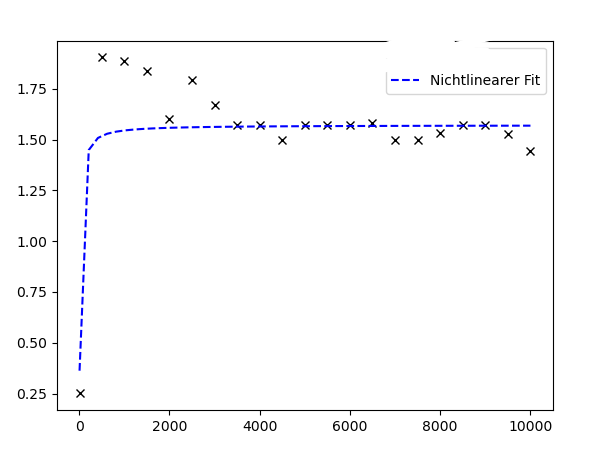
\includegraphics[width=\textwidth]{build/plot1.pdf}
  \caption{Messdaten und Fehlerbalken der Geiger-Müller Charakteristik}
  \label{fig:plot1}
\end{figure}

\subsection{Bestimmung der Totzeit}

\subsubsection{Ablesen am Oszilloskop}
blablabla

\subsubsection{Zwei-Quellen-Methode}
Anhand der Zwei-Quellen-Methode lässt sich die Totzeit $T_{tot}$ des verwendeten Zählrohrs mit Gleichung \eqref{eqn:totzeit} bestimmen.
Zusammen mit der Fehlerbehaftung der Messwerte nach der Poissonverteilung \eqref{eqn:fehlerzählrate} lässt sich nun wieder eine
Gaußsche Fehlerfortpflanzung formulieren.

\begin{equation*}
\increment T_{tot} = \sqrt{\left( \frac{N_{1+2} - N_{2}}{2 N_{1}^{2} N_{2}}\right)^2 \cdot (\increment N_{1})^{2} 
\left( \frac{N_{1+2} - N_{1}}{2 N_{2}^{2} N_{1}}\right)^2 \cdot (\increment N_{2})^{2} 
\left( \frac{1}{2 N_{1} N_{2}}\right)^2 \cdot (\increment N_{1+2})^{2}} 
\end{equation*}

Hier werden die Werte aus der Tabelle \ref{tab:ogemessdaten3} verwendet und vor dem Einsetzen auf $\text{Imp} / \si{\second}$ umgerechnet.
Für die Totzeit $T_{tot}$ ergibt sich nach der Zwei-Quellen-Methode folglich

\begin{equation}
T_{tot} \approx \SI{115(47)}{\micro\second}
\end{equation}